\chapter{UMBEM: Una métrica universal para comparar el desempeño de materiales de electrodos de carga rápida}\label{ch:umbem}
\thispagestyle{empty}

\vspace{50pt}

\begin{adjustwidth}{50pt}{50pt}
    En la búsqueda de una métrica universal que permita estandarizar las 
    comparaciones en el desempeño de distintos materiales con capacidad para
    aplicarse en una carga rápida, se define aquí la métrica UMBEM (
    \textit{Universal Metric for Benchmarking Electrode Materials}) como el 
    estado de la carga máxima retenida cuando el material es cargado por 15 
    minutos en condiciones de corriente constante. Esta proposición se basa 
    en un método general que considera la influencia de la difusión finita, 
    la cinética de la transferencia de carga, el tamaño de la partícula y la 
    C-rate, que ya fue introducido en el capítulo \ref{ch:un}. Además, se establece
    una jerarquía de materiales de acuerdo a su valor UMBEM y se predicen las 
    modificaciones en los parámetros requeridas para alcanzar la carga rápida.
\end{adjustwidth}

\clearpage
\newpage
\thispagestyle{empty}
\mbox{}
\newpage

Como ya se ha mencionado en esta tesis, lograr una carga rápida de una batería 
de ion-litio no es una tarea simple de realizar ya que a diferentes escalas 
ocurren distintos procesos que deben optimizarse \cite{franco2013}. En 
particular, en la escala del electrodo se tiene que las partículas se encuentran
en el orden de los nano/micro-metros y que a dicho nivel la velocidad de carga 
depende en gran medida de la difusión de iones dentro del material activo y del
intercambio de los mismo en la interfase electrodo/electrolito \cite{weiss2021}.
Mientras que el primero de los procesos mencionados puede considerarse como una 
propiedad intrínseca del material, el segundo de ellos es menos específico y, 
por lo tanto, más configurable ya que depende de muchos factores como el 
solvente \cite{levin2017}, la estructura cristalina \cite{li2022}, la
orientación de los cristales \cite{mala2020}, modificaciones en la superficie o 
distintas composiciones de electrodos \cite{kaur2022}. Con respecto al material
activo, el tamaño y la geometría de la partícula imponen las condiciones más
relevantes para el transporte de iones dentro de ellas. Otros factores como la 
composición, la porosidad, la tortuosidad y la distribución del material 
conductivo del electrodo también son importantes \cite{weiss2021}. Sin embargo,
como se mencionó en el capítulo \ref{ch:un}, si estos factores están 
optimizados, las limitaciones estarán impuestas por los anteriores. Esto último
da relevancia a un análisis del comportamiento de los materiales de electrodos
utilizando un enfoque de una sola partícula.

Al momento de la escritura de esta tesis se carece de una métrica universal 
para comparar mediciones de distintos sistemas reportados en publicaciones
científicas, lo cual obstaculiza el desarrollo de materiales de electrodos de
carga rápida. Sería especialmente atractivo contar con una métrica que 
estandarice las comparaciones de una manera simple y que sea capaz de realizar
predicciones fiables. Por ejemplo, una práctica usual es comparar las 
capacidades de los electrodos a una misma C-rate, pero, a pesar de que algunas
veces da una diagnostico aproximado del problema, no facilita un análisis 
integral ya que, por ejemplo, el efecto del tamaño y la geometría de las 
partículas no son tenidos en cuenta. Por otro lado, el coeficiente de difusión
suele ser reportado como un parámetro para evaluar el desempeño de electrodos,
pero por sí solo no aporta una información suficiente ya que omite la 
influencia de la cinética en la interfase. En consecuencia, una métrica fiable 
debe tener en cuenta todos estos factores y la relación entre ellos. Un avance
reciente en esta dirección ha sido realizada por Xia \textit{et al} 
\cite{xia2022} en un artículo de perspectiva. Los autores presentaron una 
figura de mérito (FOM, \textit{Figure of Merit}) para estandarizar las 
comparaciones de los materiales de baterías de carga rápida. Esta FOM combina
los efectos de los coeficientes de difusión y los tamaños de las partículas 
para calcular el tiempo característico de difusión como un parámetro 
fundamental para la evaluación del cargado rápido. Para obtener este parámetro,
suponen una transferencia de carga extremadamente alta y una geometría plana 
en condiciones de difusión semi-infinita. En sus conclusiones, los autores 
expresaron la necesidad de refinar este modelo para mejorar el diagnóstico. 
El objetivo de este capítulo es proponer la métrica UMBEM (\textit{Universal
Metric for Benchmarking Electrode Materials}) para materiales de carga rápida
de baterías de ion-litio en condiciones de cargado galvanostático. Con este
objetivo, se considera una difusión finita y una cinética en la interfase 
controladas por cuatro parámetros: el coeficiente de difusión de los iones 
dentro del material ($D$), la constante cinética de transferencia de carga
($k^0$), la C-rate ($C_r$) y el tamaño de partícula ($d$).

El método utilizado ya fue explicado en la sección \ref{s:metodologia} del
capítulo \ref{ch:un}, un resumen de la explicación del mismo se encuentra 
en la Figura \ref{fig:explicacion}. En la Figura \ref{fig:explicacion}a se 
muestra un esquema del modelo de una sola partícula para obtener el estado
de la carga del material en cuestión. Luego, la utilización de dos parámetros
$\Xi$ y $\ell$ adimensionales, resumidos en la Figura \ref{fig:explicacion}b,
permiten la construcción de un diagrama universal (Figura 
\ref{fig:explicacion}c), que se extendió con respecto al capítulo \ref{ch:un}
y se seleccionó un potencial de corte de 200 mV. Esto lo que permite es 
calcular la UMBEM como el SOC máximo alcanzado cuando el material es cargado
en 15 minutos en condiciones de carga constante; una ilustración de esta 
definición se presenta en la Figura \ref{fig:explicacion}d, la cual muestra 
el comportamiento cualitativo de un perfil galvanostático típico. La UMBEM
es igual a 1 cuando el electrodo se encuentra completamente cargado, tiene
un valor $\geq 0$ cuando satisface el criterio del USABC \cite{USABC} y
valores menores (hasta 0) cuando el material no califica como de cargado 
rápido dadas las condiciones definidas. La curva verde representa el caso 
UMBEM$ = 0.8$, mientras que la violeta un caso de UMBEM$ = 0.3$ La UMBEM 
pretende estandarizar las comparaciones entre el desempeño de distintos 
materiales para considerarse en una aplicación de carga rápida de electrodos
de baterías de ion-litio, también permite establecer una jerarquía de 
materiales de acuerdo a su valor.
\begin{figure}[h!]
    \centering
    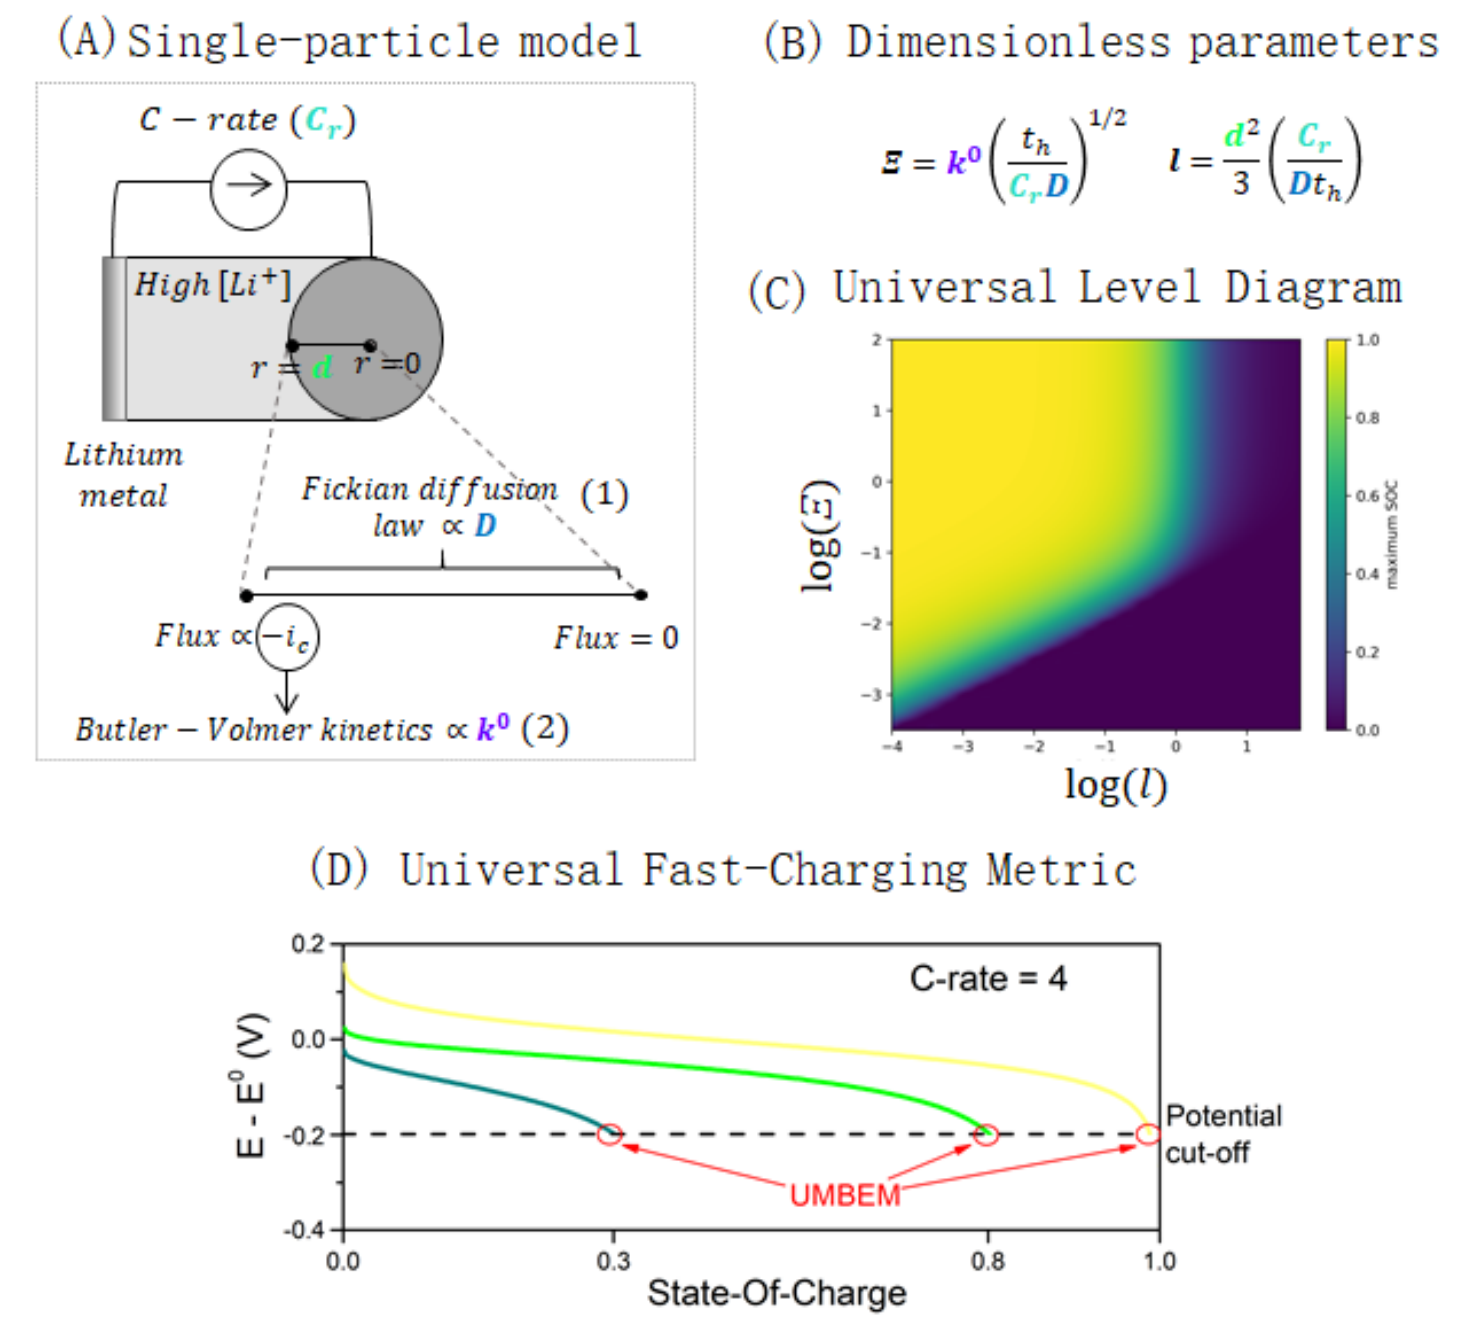
\includegraphics[width=\textwidth]{FastCharging/umbem/explicacion.png}
    \caption{Esquema del modelo utilizado para construir el diagrama y hacer 
    las predicción de carga rápida. (a) Modelo de una sola partícula. (b) 
    Parámetros adimensionales que se derivan de las condiciones del modelo 
    en la sección \ref{s:derivparam}. (c) Diagrama universal construido con 
    simulaciones galvanostáticas que representa el estado de carga alcanzado para 
    un potencial de corte de 200 mV y una geometría esférica. (d) Ilustración
    de la métrica UMBEM que se presenta en este capítulo.}
    \label{fig:explicacion}
\end{figure}

La Tabla \ref{t:dataset} resume la información experimental ($d$, $D$) que se 
requiere para evaluar con la métrica UMBEM los distintos sistemas, la misma fue 
extraída de la referencia \cite{xia2022}. Sin embargo, como la discusión se 
realizará en el contexto del modelo esquematizado en la Figura 
\ref{fig:explicacion}, también se necesita considerar la constante cinética $k^0$.
Valores experimentales típicos para este parámetro fundamental se encuentran en 
un rango que va desde $10^{-5}$ hasta $10^{-9}$ cm/s \cite{gavilan2020kinetic}, 
por lo cual se utiliza un valor intermedio de $10^{-7}$ cm/s para todos los 
materiales. La C-rate fue fijada a 4 C, que se corresponde con 15 minutos, 
de acuerdo a la propuesta del USABC. 
\begin{table}[h!]
    \centering
    \caption{Datos experimentales de distintos sistemas requeridos para evaluar 
    la métrica UMBEM.}
    \setlength\extrarowheight{2pt}\stackon{%
    \begin{tabular}{l c c l}
        \toprule
        \textbf{Material} & 
        \textbf{$d$ [cm]} &  
        \textbf{$D$ [cm$^2$/s]} &  
        \textbf{Referencia} \\ 
        \midrule
        Material & d & D & ref \\
        \bottomrule
    \end{tabular}
    }{}
    \label{t:dataset}
\end{table}
Estos cuatro parámetros se utilizan para calcular los parámetros adimensionales 
$\Xi$ y $\ell$ y así ubicar cada experimento en el mapa simulado, como se muestra
en la Figure \ref{fig:UMBEM}a. Como referencia para delimitar la región de carga
rápida del resto, se grafica la línea discontinua gris a UMBEM$ = 0.8$. Puede
resaltarse que los puntos correspondientes a una material presentan una 
dispersión mayor a lo largo del eje $\log(\ell)$ debido a la dependencia de este
parámetro con el tamaño al cuadrado de la partícula (ecuación \ref{eq:ele}). La
Figura \ref{fig:UMBEM}b muestra esta misma información en un gráfico de barras,
agrupadas por materiales. Los sistemas se encuentran ordenados por valor promedio 
por material de UMBEM decreciente. La línea discontinua horizontal es la misma que
en el diagrama, 0.8. Esto permite visualizar si el material cumple o no con el
criterio para ser clasificado como de carga rápida o no. Como se observa en las
Figuras \ref{fig:UMBEM}a y b, con la excepción de un dato, LCO y LMO se encuentran
en la región superior del mapa (UMBEM $\geq$ 0.8). Una mitad de los puntos del 
LTO y del LFP se encuentran en la zona de carga rápida y la otra mitad en la zona
de no-carga rápida. Por último, con la excepción de un caso de grafito, el grafito
y los materiales ternarios están fuera de la región de carga rápida.

\begin{figure}[h!]
    \centering
    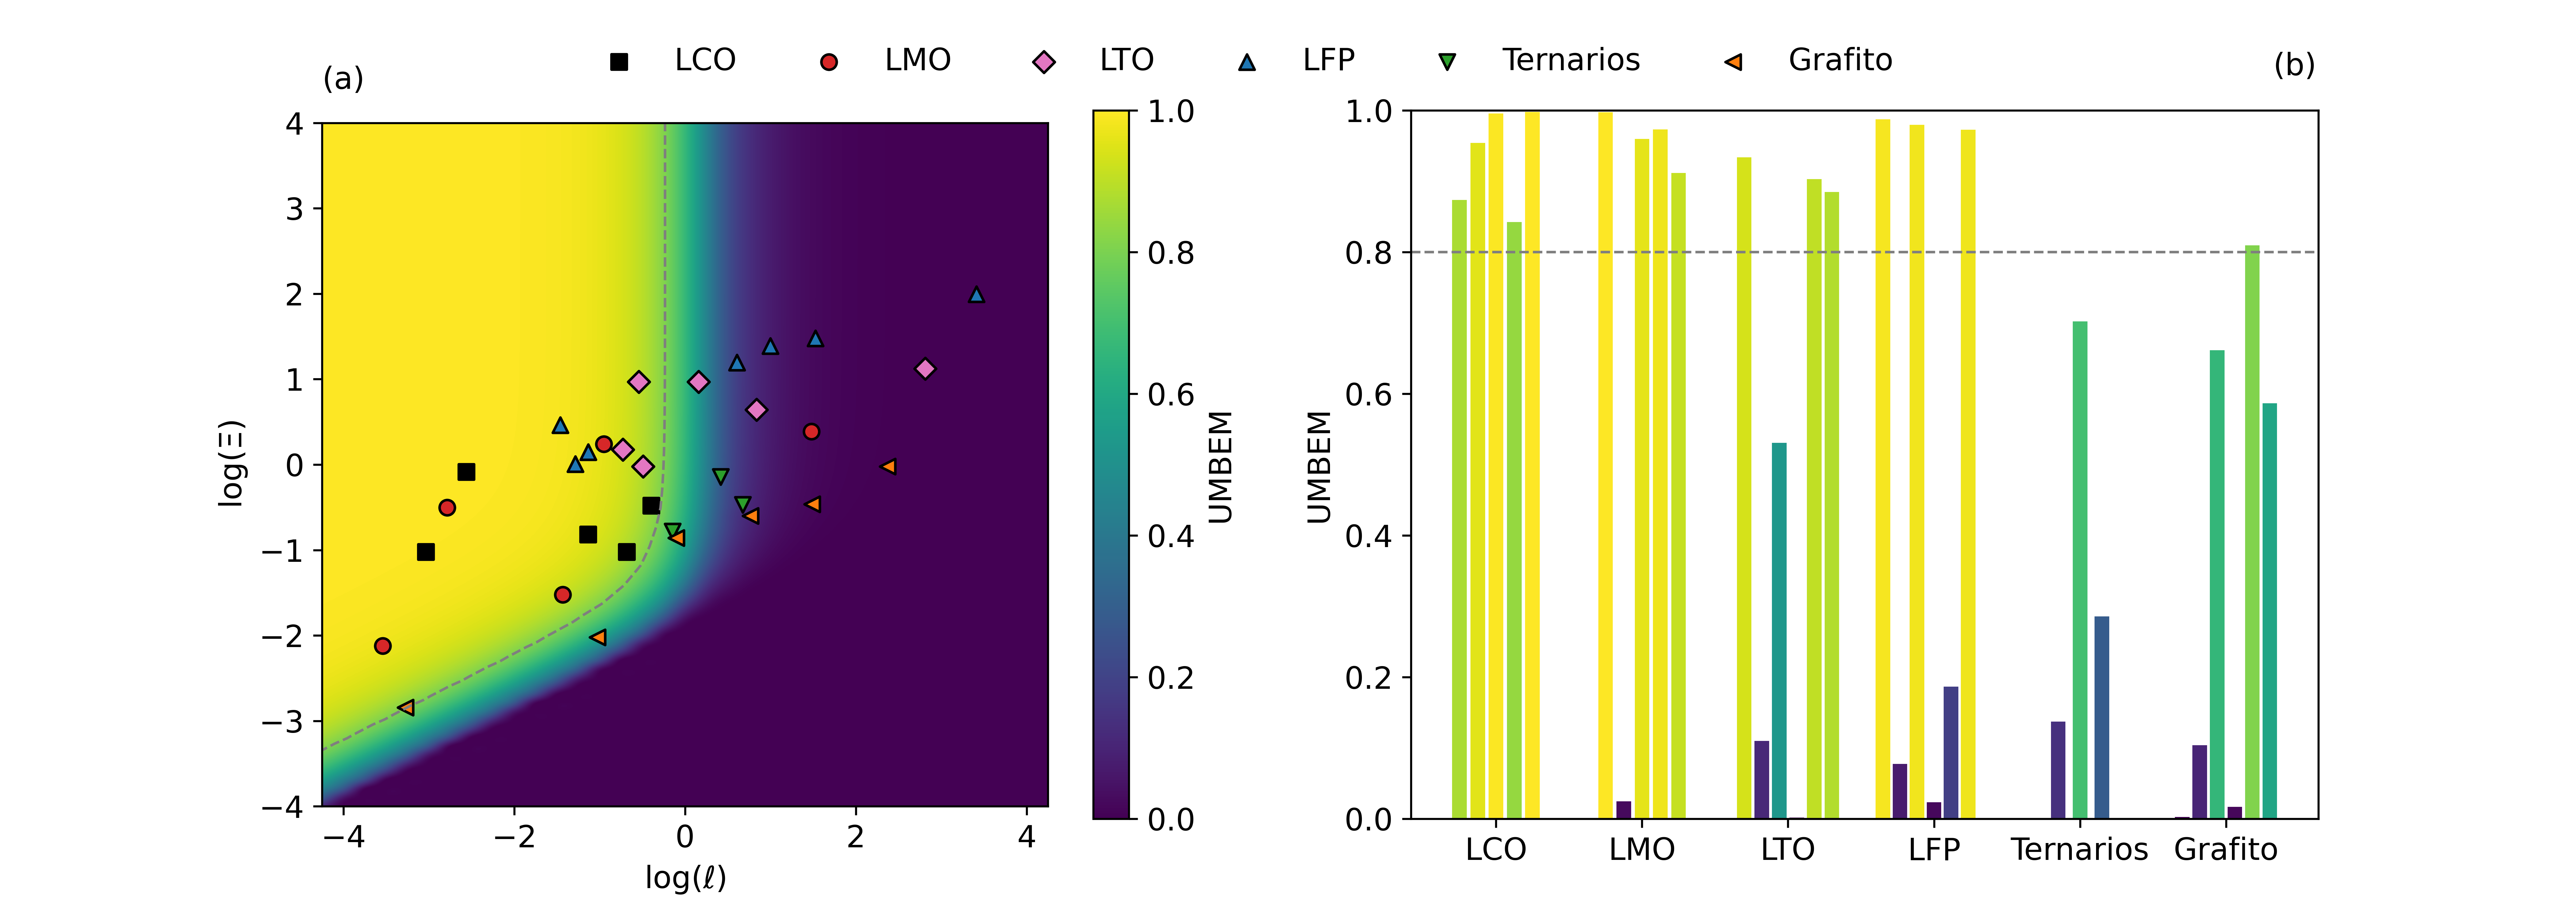
\includegraphics[width=\textwidth]{FastCharging/umbem/UMBEM.png}
    \caption{(a) Posición de cada experimento mencionado en la Tabla 
    \ref{t:dataset} en el mapa simulado representando el valor de la UMBEM. (b)
    Histograma con los valores de la UMBEM, ordenados por el desempeño promedio
    de cada sistema.}
    \label{fig:UMBEM}
\end{figure}

Xia \textit{et al} \cite{xia2022} utilizaron los datos experimentales de $d$ y $D$
que se encuentran en la Tabla \ref{t:dataset} para calcular su FOM a cada uno 
de ellos, como se muestra en los puntos de la Figura \ref{fig:xiacomp}a. Los 
valores de la UMBEM obtenidos en la Figura \ref{fig:UMBEM} son utilizados para
colorear cada uno de ellos con el propósito de comparar ambas métricas, como
se muestra en la barra de colores de la Figura \ref{fig:xiacomp}a. A continuación
se analiza si es que existe una correspondencia entre ambas métricas en 
consideración, la FOM y la UMBEM. Si hubiera una correspondencia perfecta entre
las dos métricas, todos los puntos situados a lo largo de las líneas grises 
discontinuas deberían tener el mismo color. Sin embargo, puede apreciarse como 
los puntos que se encuentran sobre una dada línea, a medida que aumenta el tamaño
de la partícula y el coeficiente de difusión, el valor de la UMBEM decrece. Por
lo cual, para una relación constante de $d^2/D$, se espera un mayor desempeño 
si tanto $d$ como $D$ son menores. Esto muestra una importancia de tamaños de 
partícula menores sobre los coeficientes de difusión mayores.

\begin{figure}[h!]
    \centering
    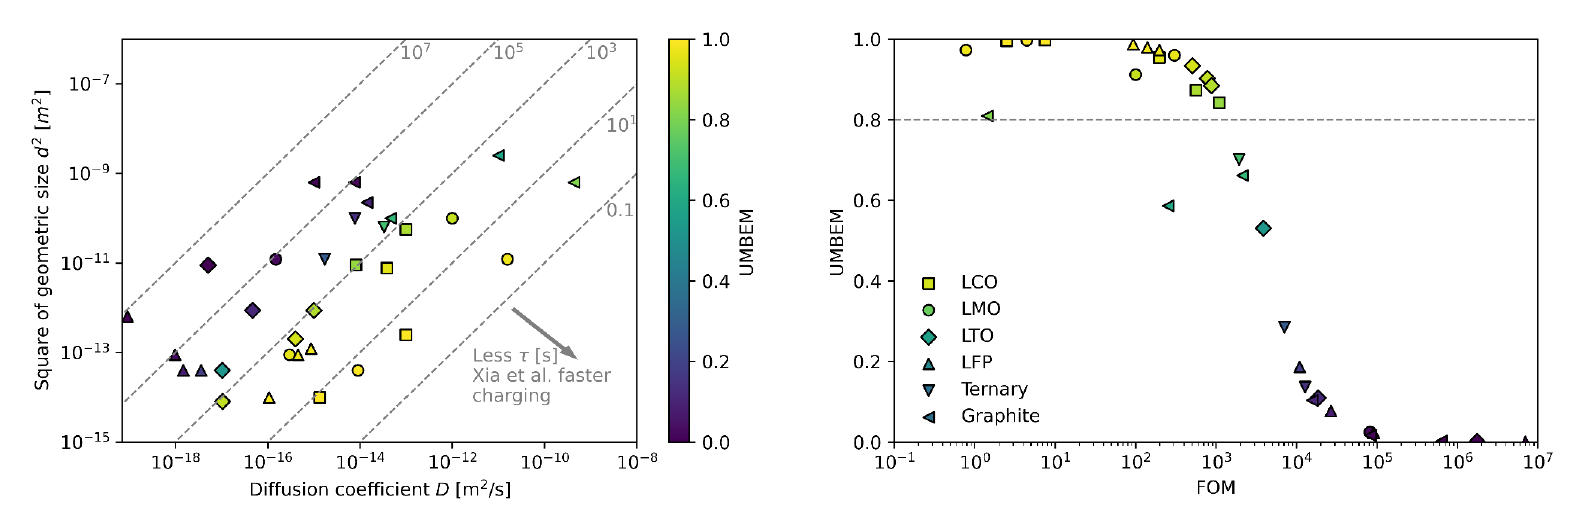
\includegraphics[width=\textwidth]{FastCharging/umbem/xiacomp.png}
    \caption{(a) Cuadro con los puntos de la Figura de Mérito (FOM) de Xia 
    \textit{et al} coloreados de acuerdo a los valores de la UMBEM. (b) UMBEM en 
    función de FOM.}
    \label{fig:xiacomp}
\end{figure}

La Figura \ref{fig:xiacomp}b presenta la UMBEM en función de la FOM para la 
elección actual de $k^0$. Se puede observar una correlación entre ambas métricas.
Puede afirmarse que un valor de FOM menor a 10$^3$ s es considerado por la UMBEM 
como carga rápida. Sin embargo, se observan algunos valores fuera de lo esperado,
especialmente en el caso del grafito que para dos experimentos dan un valor de 
FOM menor a 10$^3$ s pero un valor de UMBEM menor comparándolos con otros 
materiales como valores similares de FOM. El bajo desempeño del grafito en 
comparación a los otros materiales puede entenderse al observar los dos puntos 
del grafito que de encuentran al borde de la zona de carga rápida de la Figura 
\ref{fig:UMBEM}a. Lo cual muestra que a pesar que el valor de $d^2/D$ indica
un tiempo de carga favorable (Figura \ref{fig:xiacomp}a), el coeficiente de 
difusión mayor da un valor menor de $\Xi$ (Figura \ref{fig:UMBEM}a) que resulta
en un bajo rendimiento cinético, que no es descripto por la métrica FOM.

Otra ventaja de la UMBEM sobre la FOM es que da un valor definido entre 0 y 1,
permitiendo una estimación cuantitativa de la condición de carga rápida de un
material dado. Mientras que la FOM no tiene un valor máximo y mínimo claramente
definido, ni un valor a partir del cual clasificar un material como de carga 
rápida o no.

La Figura \ref{fig:sizes}a muestra un diagrama de nivel, indicando la zona de 
carga rápida y la de no-carga rápida separadas por una línea correspondiente a
UMBEM$ = 0.8$. Como ya se ha dicho, este es el menor valor de carga rápida 
propuesto por el USABC. Fuera de la región de carga rápida se encuentran dos 
sistemas de ejemplo (cuadrado y círculo rojos) para dar una idea cualitativa de 
cómo un análisis guiado por el mapa puede ayudar a optimizar el desempeño de 
estos sistemas. El cuadrado que se encuentra abajo a la izquierda del gráfico 
podría desplazarse verticalmente para alcanzar la línea divisoria. Para que 
ese desplazamiento ocurra se necesitaría un aumento en $k^0$, como detalla la 
flecha apuntando hacia arriba en la Figura \ref{fig:sizes}a. Con respecto al 
círculo que se encuentra arriba a la derecha, se muestran dos opciones para
optimizarlo. Una consiste en moverse horizontalmente hacia la izquierda en el 
diagrama, lo cual puede lograrse reduciendo el tamaño de la partícula, como 
se muestra con la flecha horizontal etiquetada con el símbolo $d$. La otra opción
es moverse en diagonal por un incremento en el coeficiente de difusión, como 
muestra la flecha etiquetada con $D$. En principio, cambiar el tamaño de la 
partícula sería la más fácil de las tres opciones (cambiar $k^0$, $d$ o $D$) para 
optimizar la carga retenida, ya que experimentalmente es posible controlar este 
parámetro regulando las condiciones de síntesis de los materiales. En el parráfo
siguiente se analiza la optimización en $d$ para todos los experimentos 
considerados.

\begin{figure}[h!]
    \centering
    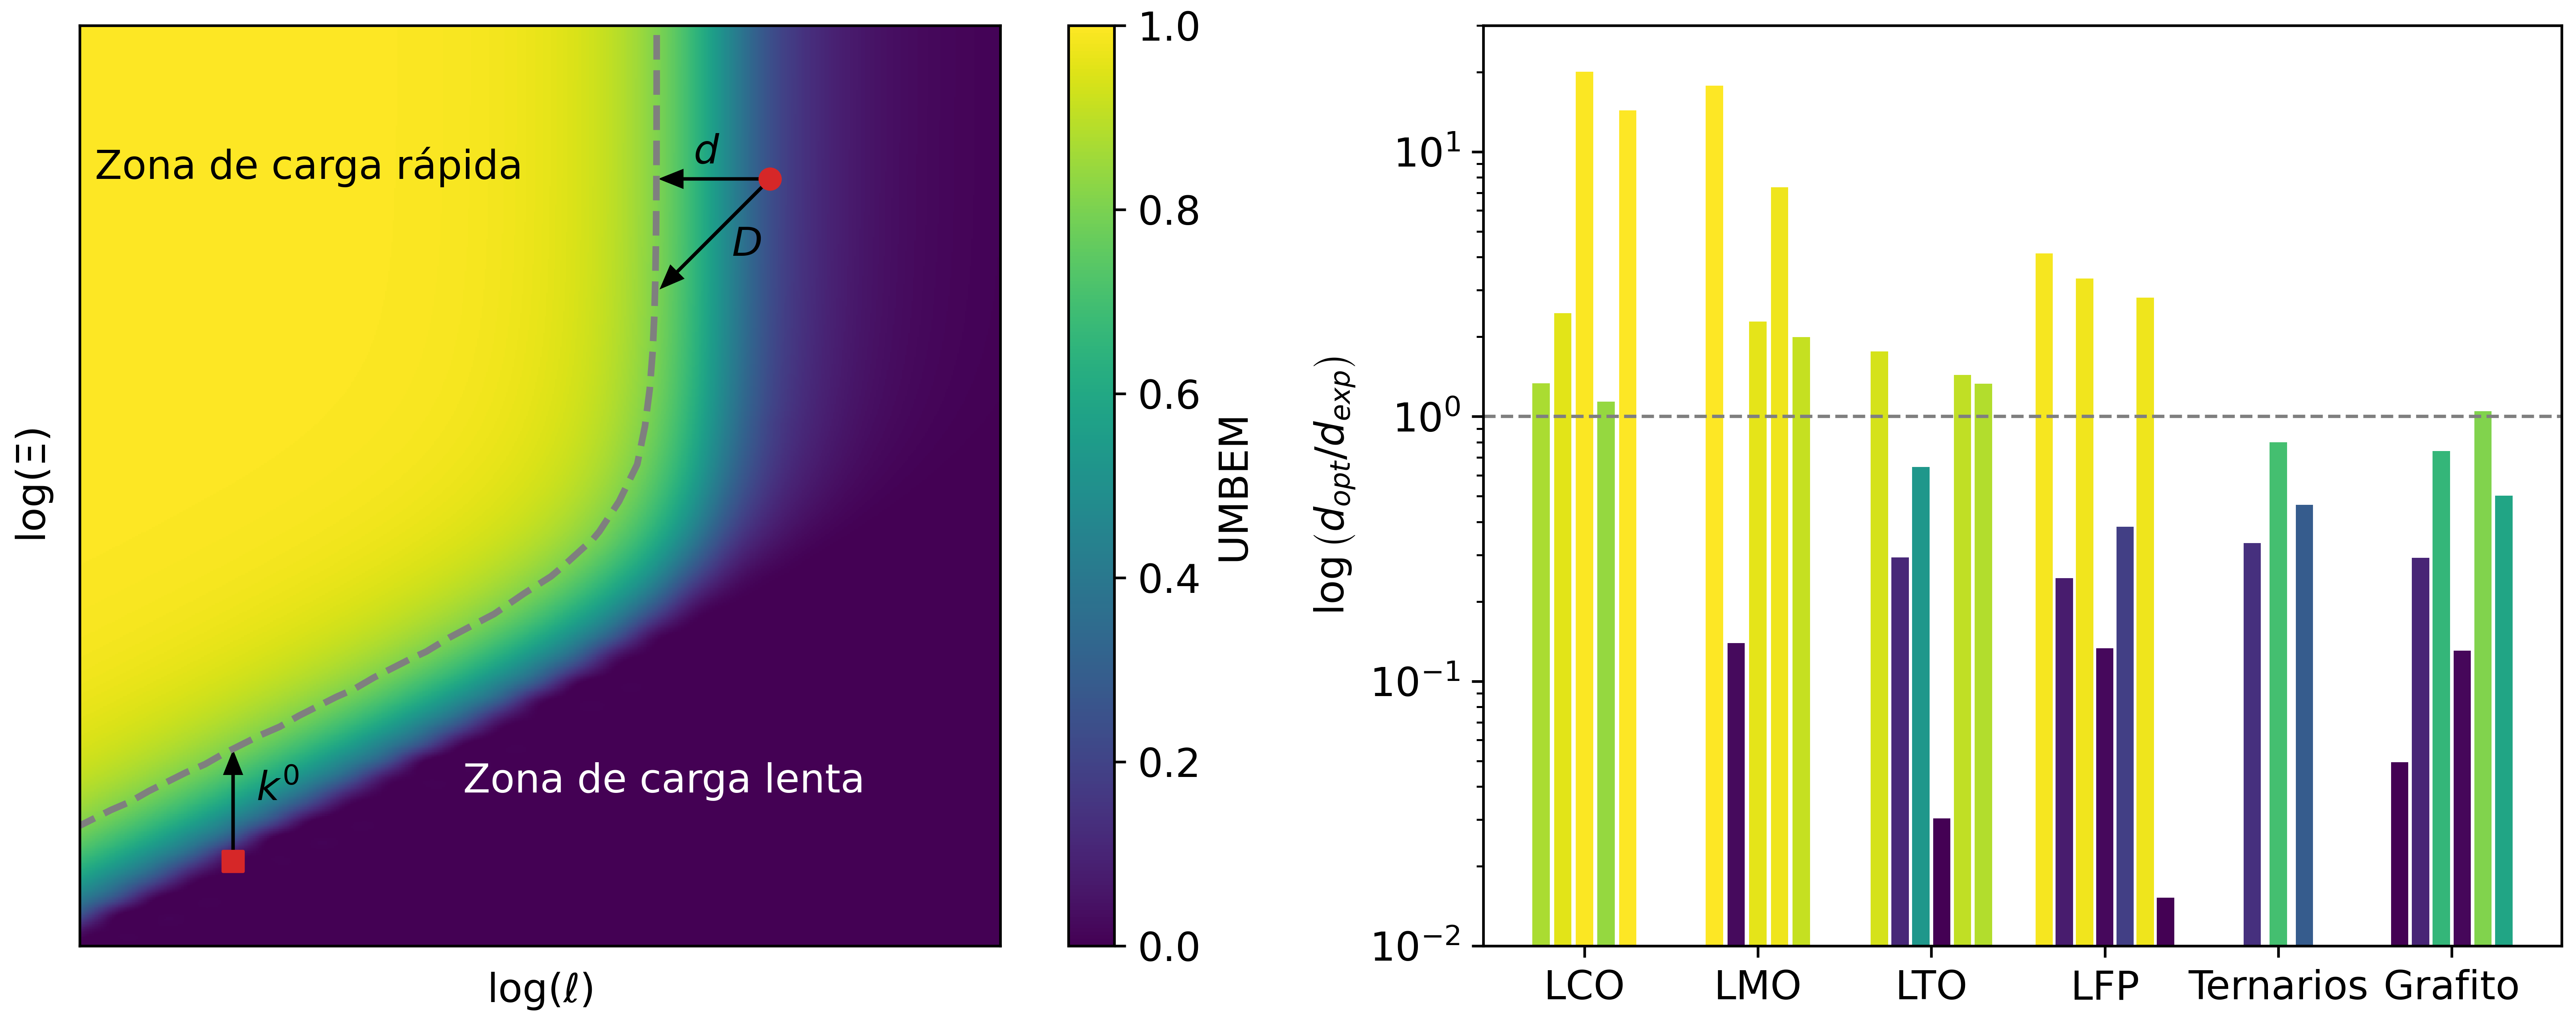
\includegraphics[width=\textwidth]{FastCharging/umbem/sizes.png}
    \caption{(a) Diagrama de las distintas maneras de optimizar el rendimiento 
    de un material. (b) Relación entre el tamaño óptimo predicho 
    ($d_{\text{opt}}$) y el experimental ($d_{\text{exp}}$) en escala logarítmica.
    El tamaño óptimo predicho es el requerido para obtener un valor de UMBEM 
    de 0.8. El color de cada barra está dado por su desempeño previo y están en 
    el mismo orden que en la Figura \ref{fig:UMBEM}a.}
    \label{fig:sizes}
\end{figure}

Se realizaron las predicciones de los tamaños óptimos de partícula para que todos 
los casos alcancen un valor de UMBEM de 0.8, tanto para aquellos que excedían 
dicho valor como para los que estaban por debajo. Esto se presenta en al Figura 
\ref{fig:sizes}b, donde se dividieron las predicciones de los tamaños óptimos 
($d_{\text{opt}}$) por los tamaños experimentales ($d_{\text{exp}}$) para permitir
una comparación mejor entre los datos de los distintos materiales. El color de 
cada barra en el histograma está dado por su desempeño original, ya que con 
el nuevo tamaño todos tendrían el mismo color correspondiente a la UMBEM de 0.8.
La línea discontinua se corresponde al cado $d_{\text{opt}} = d_{\text{exp}}$.

En este capítulo se definió una métrica universal para comparar el desempeño
de materiales de electrodos de carga rápida (UMBEM) como el estado de la carga 
alcanzado cuando el material se carga en condiciones de corriente constante 
durante 15 minutos. Esta métrica presenta una mejora sobre un trabajo anterior al
considerar la difusión finita, la transferencia de carga, el tamaño de la 
partícula y el tiempo de carga. Basándose en el valor de la UMBEM para distintas 
caracterizaciones experimentales, fue posible establecer una jerarquía de 
sistemas y predecir las mejoras necesarias para clasificarlos como materiales de 
carga rápida.
